\chapter{Studying the Higgs boson through vector boson scattering at CMS}\label{ch:higgs_vbs}
\begin{aquote}{Peter Higgs, Edinburgh University press conference, 2012}
    It's very nice to be right sometimes.
\end{aquote}

\section{New physics and the Higgs boson}
The stage is set: over a century of particle physics has yielded a beautiful theory of \textit{almost} everything, the Standard Model, and a grand coalition of nations has built the largest and most complex scientific instrument in human history, the LHC, to test it. 
The most recent act in this drama concluded in 2012, when the Higgs boson was discovered at CMS and ATLAS~\cite{CMSdisc, ATLASdisc}. 
In the years following its discovery, the LHC experiments have measured many of its properties to great precision and found no significant deviations from SM predictions~\cite{NatureHiggsCMS2022, NatureHiggsATLAS2022}. 
However, there are many features yet to be measured precisely. 
This implies that studies of the Higgs boson have incredible potential for discovery: a better understanding of the Higgs boson immediately yields a better understanding of the origin, operation, and continued existence of the entire universe. 
Moreover, the Higgs boson can uniquely interact with all known matter, so by producing many Higgs bosons in the lab, we may be able to access physics beyond the Standard Model (BSM). % citation needed

There are many educated guesses, called theories, as to the mysterious nature of the Higgs boson. 
Some guess at the existence of yet-undiscovered particles that also interact with the Higgs boson\footnotemark{}, and experimentalists can search for their existence directly: either by looking for the SM particles that they might decay into, or by checking for what is missing after everything is else accounted for. 
\footnotetext{This is not an unlikely guess: dark matter is known to have mass, and it may haved obtained that mass through the Higgs mechanism.}
Experimentalists can also search for new physics indirectly by making precise measurements of SM predictions; any significant deviation from the prediction would poke another hole in the Standard Model or even confirm a prediction of a new theory. 
The physics analyses described in this document both follow the latter strategy.

\subsection{The $\kappa$-framework}
One commonly used framework used to quantify these deviations from the SM is the so-called $\kappa$-framework~\cite{KFrame}, which introduces modifiers $\kappa_X$ to the Higgs boson couplings to some particle $X$:
\begin{equation}
    \kappa_X = \frac{\text{modifed coupling value}}{\text{SM coupling value}}.
\end{equation}
While there are myriad theoretical nuances to the statement above, it is sufficient to state the obvious: $\kappa_X = 1$ represents the SM scenario and significant deviations from 1 represent BSM scenarios. 
The $\kappa$-framework is not the only framework used to understand and quantify modifications to the SM, however, with the most notable alternative being Effective Field Theory~\cite{EFT, DimSix}. 

\section{Producing Higgs bosons with vector boson scattering}
The dominant Higgs boson production mechanism at the LHC is gluon-gluon fusion through a top quark loop. % TODO: add feynman diagrams, cite PDG?
Through these processes, the Higgs boson was discovered and many of its branching ratios and couplings have been measured precisely. 
However, additional production mechanisms can yield unique insights. 
Enter vector boson scattering\footnotemark{} (VBS), where two quarks scatter off of each other by the exchange of vector bosons ($\PV = \PW$ or \PZ). % TODO: add feynman diagram, ideally with "here there be monsters" circle with stuff coming out
\footnotetext{Although VBS specifically implies the production of two vector bosons, while vector boson fusion (VBF) implies the production of a single Higgs or vector boson~\cite{RauchVBSVBF2016}, the names VBS and VBF are used interchangeably; since we are interested in the production of a Higgs boson and one or two vector bosons, the naming is anyway ambiguous.}
This exchange can, in turn, produce a variety of physics, most notably the production of at least one Higgs boson. 
This process also has two important features. 
First, it has a unique signature: the two scattered quarks fly out of the collision back-to-back, typically in the forward regions of the detector (Fig.~\ref{fig:vbs_fireworks}), with a large energies. 
Second, but equally important, modifications to the Higgs couplings induce effects that grow with energy~\cite{HiggsWithoutHiggs}---at the LHC, where energy is plentiful, this makes BSM scenarios easier to spot. 

\begin{figure}[htb]
    \centering
    \subfloat{\includegraphics[width=0.45\textwidth]{fig/vbswh/fireworks/signal/vbswh_evt131104_rz_gen_labeled.png}}\qquad
    \subfloat{\includegraphics[width=0.45\textwidth]{fig/vbswh/fireworks/signal/vbswh_evt131104_rz_gen_labeled.png}} % TODO: label another plot, maybe VBSVVH, and replace this one
    \caption{
        Event display for a simulated VBS WH signal event. 
        The event is shown in the x-y plane (left) and x-z plane (right), and the final-state particles (thick red lines) are labeled with their true labels. 
        Two VBS jets can be seen very near to the beamline, going in either direction in $z$. 
    }
    \label{fig:vbs_fireworks}
\end{figure}

VBS provides a unique way of producing Higgs bosons, with an easily identifiable signature, and there are myriad VBS processes involving a Higgs, each involving different couplings. 
The rarer couplings are of particular interest, including the $\HHVV$ and $\HHH$ couplings (Ch.~\ref{ch:vbsvvh}). 
Also of interest are some of the more obscure properties of the Higgs boson, like the relative sign between the $\HWW$ and $\HZZ$ couplings (Ch.~\ref{ch:vbswh}). 
In all of these measurements, if we confirm SM predictions, we exclude possible BSM directions, and if find a significant deviation from the SM, we will have opened an entirely new chapter of physics. 

We begin by selecting the Feynman diagrams that involve the couplings of interest---here, we focus on VBS processes. 
We call the selected processes our ``signal.'' 
For example, if we are interested in $\HHVV$, as in Ch.~\ref{ch:vbsvvh}, our signal might be VBS production of a Higgs boson and two vector bosons. 
We must then find our signal, which is often incredibly rare, amongst petabytes of data recorded by CMS. 

\section{Choosing a final state}
The final collection of particles that are actually recorded by CMS are called the ``final state.'' 
As covered in Chapter~\ref{ch:lhc_cms}, Section~\ref{sec:cms}, CMS can record electrons, photons, hadrons, and photons. 
All other SM particles---including Higgs bosons, vector bosons, and gluons---decay to these particles, and we hope that BSM particles might as well. 
Importantly, SM particles can also decay to neutrinos, which pass through CMS completely undetected, and it is possible that BSM particles are similarly missed. 
The presence of these particles can be inferred, however (Sec.~\ref{sec:met}). 

When we say we are looking for VBS production of a Higgs boson and two vector bosons, for example, we are really looking for two quarks (VBS) and the decay products of the bosons. 
Some final states are preferable over others, however. 
For convenience, we often prefer to look for \Htobb, since a Higgs boson is most likely to decay to \bbbar (i.e. \Htobb has the highest ``branching ratio''). 
The choice for the decay of the vector bosons is less clear. 
The leptonic decays ($\PW\to\Pell\PGn$ or $\PZ\to\Pellp\Pellm$) are easier to spot, but are more rare. 
On the other hand, the hadronic decays ($\PV\to\qq$) are more plentiful, but are difficult to distinguish from far more abundant processes. 

\section{Reconstruction}
The subdetectors that comprise CMS produce a set of electric signals digitized into data that can be used as measurements of physical quantities. 
Moreover, when associated to one another, these measurements can also be used to ascertain the identity of detectable throughgoing particles (Fig.~\ref{fig:cms_particle_id}). 

\begin{figure}[htb]
    \centering
    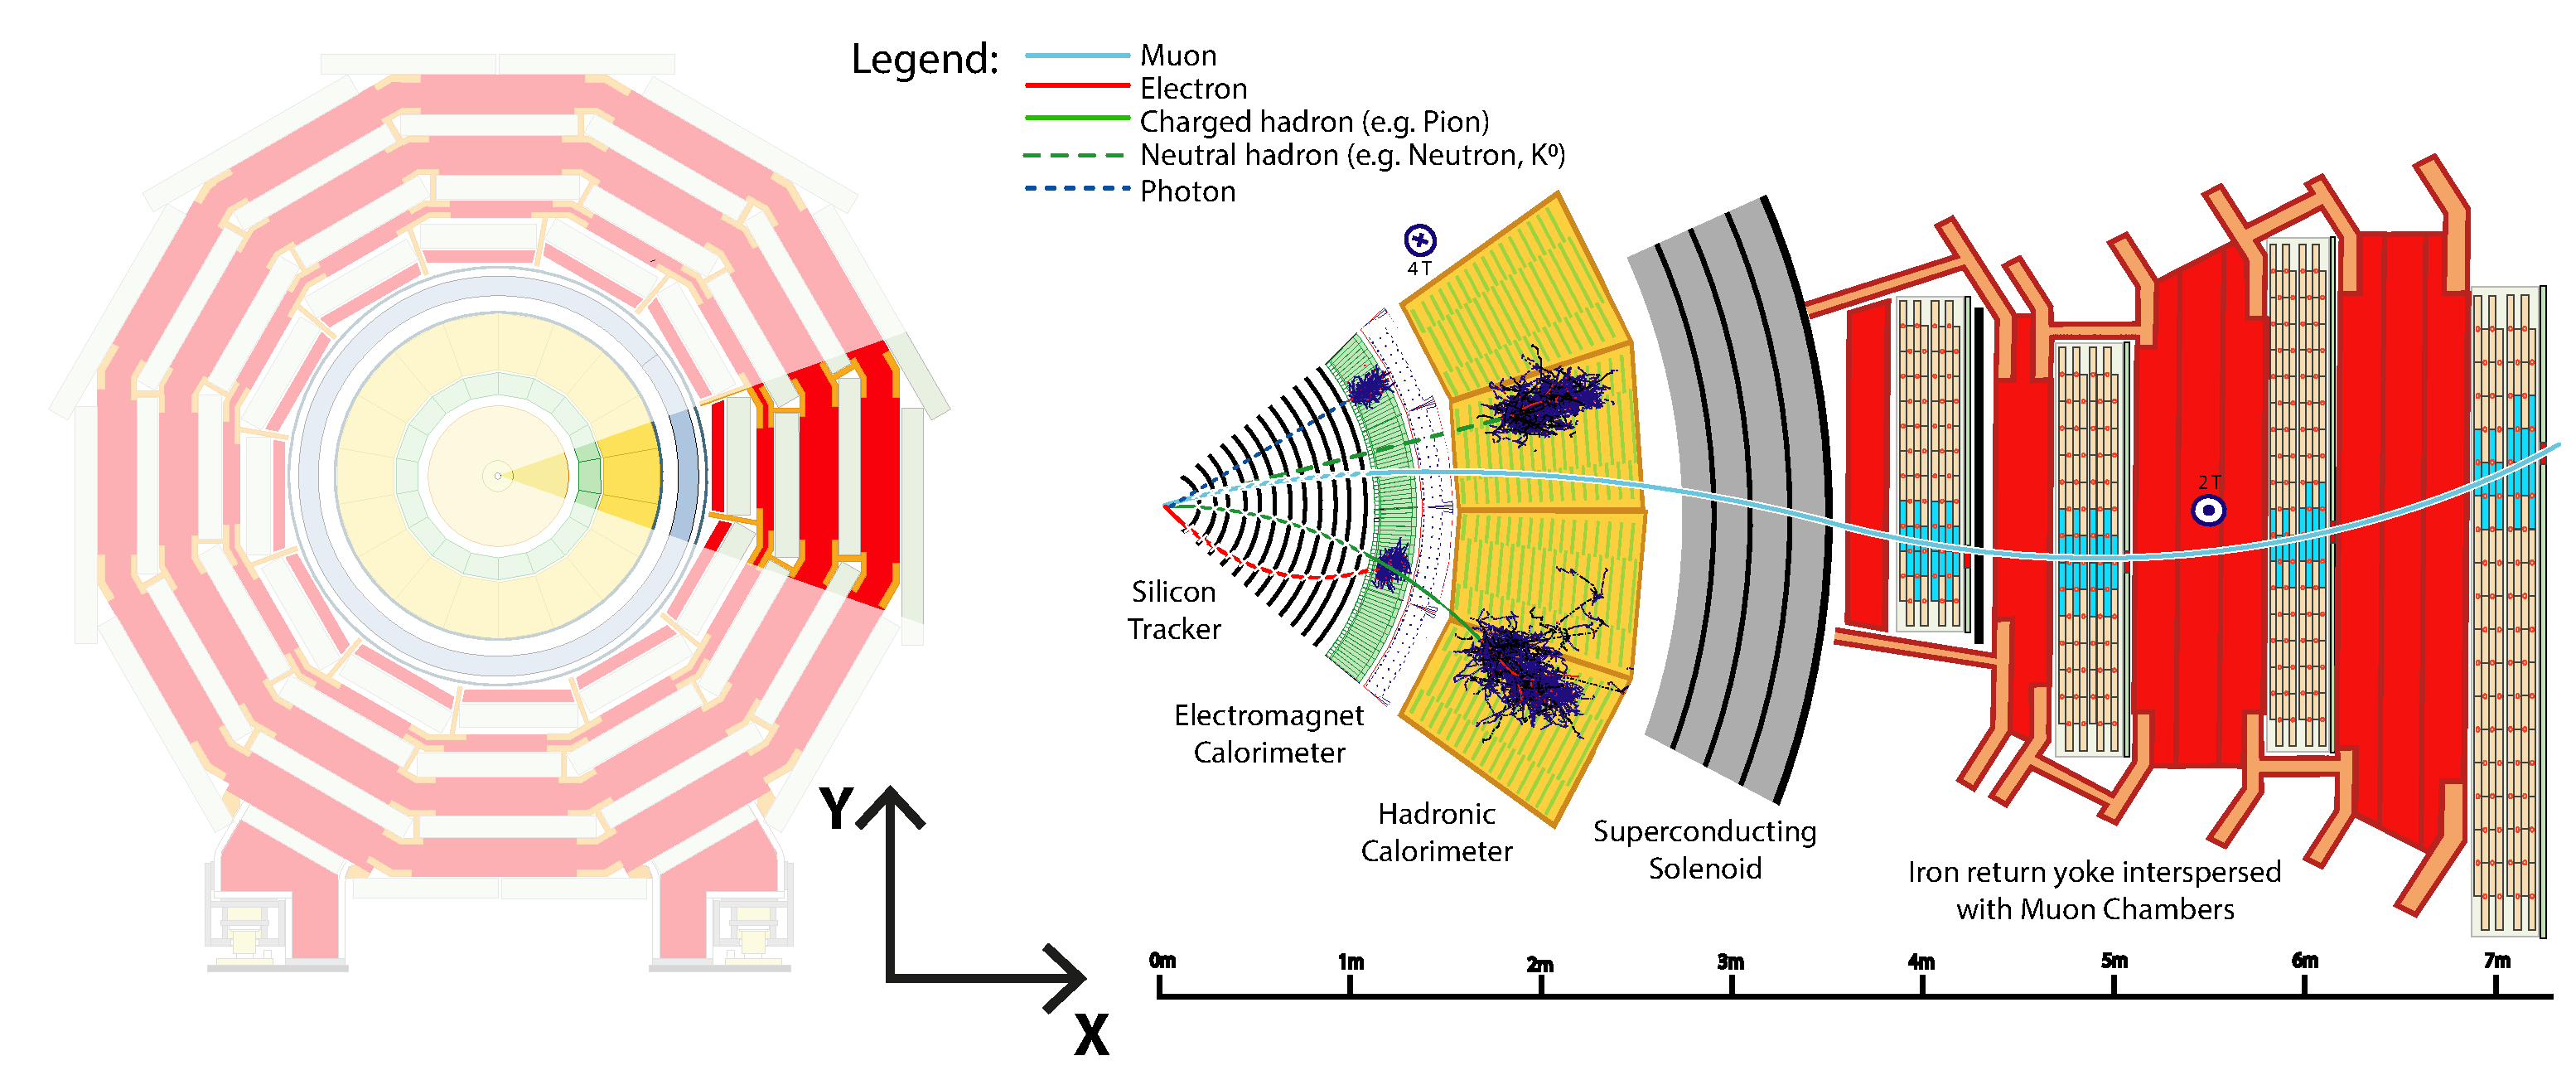
\includegraphics[width=0.95\textwidth]{fig/cms/particle_id_slice.pdf}
    \caption{
        Transverse slice of CMS, from Ref.~\cite{Davis:2205172}, showing the signals left by different kinds of particles in each subdetector.
    }
    \label{fig:cms_particle_id}
\end{figure}

\subsection{Jets}
All hadrons leave a hit in the HCAL, while charged hadrons also have a track that can be associated to it. 
These hits do not correspond to individual quarks---like the VBS quarks, for example. 
Due to quark ``confinement,'' quarks hadronize into ``jets'' of hadrons. 
This happens in a cascade, where quarks beget quarks that beget more quarks and so on, until the jet impinges on the calorimeters. 
Fortunately, jets tend to be concentrated in relatively narrow cones, meaning individual jets---and thus, individual quarks---can usually be distinguished from one another. 
Jets are constructed using the anti-\kt algorithm~\cite{Cacciari:2008gp, Cacciari:2011ma}, which clusters deposits in the calorimeters according to a configurable ``distance parameter,'' which determines the size of the jet cone. % TODO: add a diagrame of a cone in CMS coordinates
For normal jets, the distance parameter is set to 0.4, corresponding to $\DeltaR = 0.4$, where
\begin{equation}
    \DeltaR = \sqrt{\Delta\phi^2 + \Delta\eta^2}
\end{equation}

\subsubsection{Jets originating from \Pb quarks}
While the presence of quarks can be inferred from the presence of jets, the identity (flavor) of each quark is less obvious. 
However, when \Pb quarks hadronize, they produce a B meson (Fig.~\ref{fig:btagging_step1}). 
The B meson lifetime is sufficiently long such that it passes the first few layers of the tracker before decaying---only picoseconds after it was produced. 
When it decays, it produces several quarks and, potentially, a lepton. 
This results in ``displaced'' tracks in the tracker that point to a ``secondary vertex'' (Fig.~\ref{fig:btagging_step2}) as opposed to the ``primary vertex,'' or the original pp collision. 
The presence of a secondary vertex within a jet therefore gives a unique indication that it originated from a \Pb quark (Fig.~\ref{fig:btagging_step3}). 
Particle tracks are therefore vital for \Pb-tagging, so \Pb-tagged jets must be within the fiducial region of the tracker ($\abs{\eta} < 2.5$). 
For CMS analysis, a deep neural network called \DeepJet was trained to use the presence of a secondary vertex, along with additional kinematic information about the jet and its constituents, to ``tag'' jets as originating from a \Pb quark~\cite{Bols:2020bkb}. 

\begin{figure}[htb]
    \centering
    \subfloat[]{\includegraphics[width=0.28\textwidth]{fig/cms/btagging_step1.png}\label{fig:btagging_step1}}\qquad
    \subfloat[]{\includegraphics[width=0.28\textwidth]{fig/cms/btagging_step2.png}\label{fig:btagging_step2}}\qquad
    \subfloat[]{\includegraphics[width=0.28\textwidth]{fig/cms/btagging_step3.png}\label{fig:btagging_step3}}
    \caption{
        A sketch of the hadronization of a \Pb quark (left), the subsequent hadronization of the produced B meson (center), and the identification of each jet (right). 
    }
    \label{fig:btagging}
\end{figure}

\subsubsection{Merged jets originating from \Htobb}
In cases where a highly energetic particle decays to a pair of quarks, the resulting jets overlap or are near enough to each other to be difficult to separate. 
This presents a unique signal: the two nearby jets can instead be found as a single, large-cone jet. 
At CMS, a separate collection of jets is created, where the anti-\kt algorithm is used with a wider distance parameter---0.8, rather than 0.4. 
In the work presented in this dissertation, we search for Higgs bosons decaying to \bbbar at high energies, tagged as a single merged jet. 
This is made possible by a graph neural network, called \ParticleNet, trained for CMS analysis to identify the origins of merged jets based on the properties of its constituents, arranged in a graph-like data structure according to their proximity to one another~\cite{Qu:2019gqs}. 
Similar to \Pb-tagging, merged jets considered for \Xtobb tagging, for instance, must be within the fiducial region of the tracker. 
The merged jet with a mass similar to the Higgs boson, and a highest \ParticleNet \Xtobb score is considered as the best Higgs boson candidate.

\subsubsection{Jets originating from VBS quarks}\label{sec:vbsjets}
The presence of VBS quarks is inferred from the presence of two jets that are back-to-back. % TODO: add event display or something showing this, maybe detajj histogram
In events where there are more than two additional jets that do not overlap with the Higgs boson candidate jet, the two best VBS jet candidates must be selected. 
A unique VBS selection technique was derived for the work presented in this dissertation: 
if all of the jets are in one hemisphere of $\eta$, then the two jets with the largest momenta are selected; 
otherwise, the jet with the largest momentum in each $\eta$ hemisphere are selected. 

\subsection{Leptons}
For simplicity, when we consider ``leptons,'' we will exclusively mean those leptons that are directly detected by CMS, namely electrons and muons. 
Electrons have a track in the silicon tracker and leave a deposit in the ECAL. 
The tracks and ECAL deposit can be associated to one another, distinguishing electrons from photons, which only leave a deposit in the ECAL. 
Muons also have a track, but they fly past both calorimeters undetected and leave hits behind in the muon chambers. 

In the SM, the lepton family also includes tau leptons and neutrinos. 
Tau leptons decay almost immediately to hadrons or to a tau neutrino and \PW boson. 
The latter decay is difficult to reconstruct, because it is easily confused with a lone \PW boson. 
The hadronic decay, however, has a unique ``multi-prong'' structure, allowing it to be distinguished from other jets. 
Neutrinos, meanwhile, pass through the entire detector. 

\subsection{Missing energy}\label{sec:met}
Protons collide along the beamline with equal but opposite momenta so the system has a total momentum of zero. 
Because of the conservation of momentum, the sum of the momenta of all produced particles must still be zero. 
This is as true in the classical world as the quantum world. 
The shrapnel from two colliding bullets, for instance, is thrown from the collision in a disk, so the total momentum is conserved~\cite{SmarterEveryDayBullets}. 
Therefore, if an invisible particle (a neutrino or possibly something new) is produced, its momentum will not be recorded, and the sum of momenta will be non-zero. 
Since the missing momentum will be entirely in the transverse plane, the plane perpendicular to the beamline, it is referred to as \ptmiss, or missing transverse momentum. 

\section{Simulation}

\section{Identifying backgrounds}
Of course, final states are not unique. 
For example, if we were searching for $\PZ\to\Pellp\Pellm$, and thus asked for collision events with two leptons with opposite charge, we would also get events where a \PWp and \PWm were produced and both decayed leptonically. 
We could also pick up events where \PW and \PZ boson were produced, and both decayed leptonically, but the lepton from the \PW was not recorded by CMS. 
These processes that produce the same final state, but are not the signal, are referred to as ``backgrounds.'' % TODO: add details about common VBS backgrounds (ttbar), hadronic backgrounds (QCD), and so on

\section{Event selection}
In order to isolate the signal, we must place a set of selections on our data that prefer events that look like signal. 
We do this in a particular order, however, because of the sheer size of our data. % TODO: maybe add a diagram here, showing some sort of cut flow for data and MC

We first select the HLT paths most relevant to the chosen final state. 
For example, if the final state includes one lepton---say, from the leptonic decay of a \PW boson---then then we would select the single-lepton HLT paths. 
This isolates a portion of the petabytes of CMS data that are relevant for analysis. 
The HLT paths are also implemented in the simulation, so we will require that simulated events pass the same HLT paths as the data. 

Next, a series of selections are placed on the events passing the HLTs in order to narrow in on a set of events most relevant for analysis. 
For VBS Higgs boson analyses, these will select for at least two jets that look like VBS jets, and \Htobb reconstructed as one merged jet or two separate jets. 
These selections are referred to as the ``Preselection'' in this dissertation. 

The final set of selections are optimized using events that pass the Preselection. 
The simplest analyses, like that presented in Chapter~\ref{ch:vbswh}, these selections will be on properties of each particle in the signal final state. 
Other analyses, like that presented in Chapter~\ref{ch:vbsvvh}, use these variables as input to a machine learning algorithm trained to select signal events. 
Ultimately, we select a final set of events that comprise the so-called ``signal region.'' 
We will compare the number of actual collision events that enter this region to the number of events predicted by simulation. 
However, we must first derive the best possible estimate of the background in this region and compute all relevant systematic uncertainties. 

\section{Background estimation}
Although the predicted number of background events in the signal region can be taken directly from the simulation, the simulation is not perfect. 
Instead, there is a strategy---the famous ``ABCD'' method---in which only real data is used. 
First, we must identify two uncorrelated selections among those that define the signal region. 
Those selections can then be used to define regions A, B, C, and D, where region A is the signal region and regions B, C, and D have one selection, the other selection, and both selections inverted, respectively. 
Then, provided that the two selections are indeed decorrelated and that there is sufficiently little signal in regions B, C, and D, the predicted yield in region A can be computed as follows:
\begin{equation}
    \AdataPred = \Bdata\times\frac{\Cdata}{\Ddata}
\end{equation}
\noindent where \AMC, \BMC, \CMC, and \DMC are the simulated background yield in region A, B, C, and D, respectively, and \Adata, \Bdata, \Cdata, and \Ddata are the yields in data. 
By estimating the background yield in the signal region in this way, we avoid computing relying on imperfect simulation.

\section{Systematic uncertainties}
Since the background estimation strategy is data-driven, the systematics on the simulation, which are more numerous, only need to be evaluated for the signal yield. 
Most sources of systematic uncertainty are derived by varying individual theoretical scales and experimental corrections by one standard deviation and taking the maximal difference in yield as the error. 
In particular, the corrections and their uncertainties are typically derived centrally in order to augment the efficiency of a specific selection in MC to match that measured in data.
In general, these corrections are applied as an event weight $\omega$, such that the weighted contribution $\Omega$ of each raw Monte Carlo event is given by the product of the event weights for that same event. 
The yield in a given signal region $y$ containing $N$ raw Monte Carlo events is therefore given by
\begin{equation}
    y = \sum_{i = 1}^{N}\Omega_i
\end{equation}
Then, the yield $y_\text{var}$ is computed after applying a systematic variation (up or down) of each source of systematic uncertainty independently:
\begin{equation}\label{eq:systs}
    y_\text{var} = \sum_{i = 1}^{N}\Omega_i\times\frac{\omega_\text{var}}{\omega}
\end{equation}
Finally, the maximum of the percent differences $\delta_\text{up}$ or $\delta_\text{down}$ are taken as the systematic uncertainty for that source, where
\begin{equation}
    \delta_\text{var} = \bigg| 1-\frac{y_\text{var}}{y} \bigg|
\end{equation}

\section{Statistical interpretation}
\subsection{Maximum likelihood estimate}
